\documentclass[]{article}
%
\usepackage[T1]{fontenc}
% T1 fonts will be used to generate the final print and online PDFs,
% so please use T1 fonts in your manuscript whenever possible.
% Other font encondings may result in incorrect characters.
%
\usepackage{graphicx}
\usepackage{tabularborder}
\usepackage{booktabs}
\usepackage{tabularx}
\usepackage{float}
\usepackage{tikz}
\usepackage{placeins}
\usepackage{caption}
\usetikzlibrary{shapes}
\usetikzlibrary{fit}
\usepackage{fancyhdr}
\pagestyle{fancy}
\fancyhf{}
\renewcommand{\headrulewidth}{0pt}
\renewcommand{\footrulewidth}{0pt}
\fancyfoot[C]{\thepage}
\usepackage{graphicx} % Para incluir imágenes
\usepackage{amsmath}  % Para matemáticas
\usepackage{pgfplots}
\usepackage{float}
\pgfplotsset{compat=1.16}
\title{\textbf{Proyecto de Simulación: Masa y Resorte}}
\author{Lucio Mansilla , Brenda Dichiara}
\date{\today}

\begin{document}

\maketitle

\section{Introducción}
En este proyecto, exploramos la dinámica de un sistema masa-resorte, con el objetivo de comprender cómo las condiciones iniciales y los parámetros del sistema afectan su comportamiento. Utilizamos el método de Euler para resolver numéricamente las ecuaciones diferenciales que describen el sistema. En este trabajo se observo cómo la masa, la constante del resorte, la resistencia al rozamiento y una fuerza externa aplicada al modelo, afectan a la posición, velocidad oscilaciones, discipación de energía y puntos de equlibrio a lo largo del tiempo.

\section{Modelo y Método de Solución}
El modelo físico que utilizamos es el de un resorte con una masa $m$ sujeta a él, una constante de resistencia del resorte $k$, una resistencia al rozamiento $b$, y una fuerza externa $F$.

\vspace{0.1cm}
\begin{center}
\begin{tikzpicture}[scale=1.5]

    % Masa
    \draw[fill=white,opacity=0.7] (2,-0.5) rectangle ++(1,1) node[midway] {$m$};
    % Resorte
    \draw[decoration={coil},decorate] (0,0) -- (2,0) node[midway, above=5mm] {$k$};
    % Pared
    \draw[very thick] (0,-1) -- (0,1);
    % Fuerza
    \draw[->,thick, red] (3,0) -- ++(1,0) node[midway,above] {$F(t)$};
    % Rozamiento
    \draw[->,thick, blue] (2,-0.5) -- ++(-0.5,0) node[midway,below] {$b$};
    % Coordenadas
    \draw[->] (0,-1) -- ++(5,0) node[below] {$x(t)$}; % posicion
    \draw[->] (0,-1) -- ++(0,2) node[left] {$y(t)$}; % velocidad
\end{tikzpicture}
\end{center}
Las ecuaciones diferenciales que modelan este sistema continuo son:
\begin{align*}
    \frac{dx}{dt} & = v \\\\ 
    \frac{dv}{dt} & = -\frac{k}{m}x - \frac{b}{m}v + \frac{F}{m}.
\end{align*}

\section{Validación del Modelo}
Para validar nuestro modelo  es necesario comparar los resultados obtenidos a través de la simulación con soluciones analíticas ya conocidas.

En particular, dado los parámetros $k = b = m = 1$, y considerando que $F(t) = 1$ junto con las condiciones iniciales $x(0) = 0$ y $v(0) = 0$, la solución analítica se expresa como sigue:

\begin{equation}
x(t) = 1 - \frac{\sqrt{3}}{3} \mathrm{e}^{\frac{-t}{2}}\sin\left(\frac{\sqrt{3}}{2}t\right)-\mathrm{e}^{\frac{-t}{2}}\cos\left(\frac{\sqrt{3}}{2}t\right)
\end{equation}

\begin{equation}
v(t) = \frac{\sqrt{12}}{3} \mathrm{e}^{\frac{-t}{2}}\sin\left(\frac{\sqrt{3}}{2}t\right)
\end{equation}

Estas ecuaciones son válidas para todo $t \geq 0$.\\

Los valores de las funciones \(x(t)\) y \(v(t)\) para \(t = 1, 5, 10\) son:
\begin{align*}
x(1) &= 1 - \frac{\cos(\sqrt{3}/2)}{\sqrt{e}} - \frac{\sin(\sqrt{3}/2)}{\sqrt{3e}} \\
v(1) &= \frac{2\sin(\sqrt{3}/2)}{\sqrt{3e}} \\
x(5) &= 1 - \frac{\cos(5\sqrt{3}/2)}{e^{5/2}} - \frac{\sin(5\sqrt{3}/2)}{\sqrt{3}e^{5/2}} \\
v(5) &= \frac{2\sin(5\sqrt{3}/2)}{\sqrt{3}e^{5/2}} \\
x(10) &= 1 - \frac{\cos(5\sqrt{3})}{e^5} - \frac{\sin(5\sqrt{3})}{\sqrt{3}e^5} \\
v(10) &= \frac{2\sin(5\sqrt{3})}{\sqrt{3}e^5}
\end{align*}



Los resultados de la simulación para los tiempos \(t = 1, 5, 10\) se muestran en la siguiente tabla:

\captionsetup[table]{
  font=small,
  labelfont=bf,
  margin={1cm, 0cm}
}

\begin{table}[H]
    \caption{Resultados de la simulación para t=1, 5, 10}
    \label{tab:time_x_v}
    \centering
    \begin{tabular*}{\textwidth}{@{\extracolsep{\fill}}|c|c|c|}
    \hline
    \textbf{Tiempo ($t$)} & \textbf{Posición ($x(t)$)} & \textbf{Velocidad ($v(t)$)} \\
    \hline
    1 & 0.340 & 0.534 \\
    \hline
    5 & 1.075 & -0.088 \\
    \hline
    10 & 1.002 & 0.005 \\
    \hline
    \end{tabular*}
\end{table}

Estos resultados muestran que la simulación proporciona valores que están en buena concordancia con las soluciones analíticas.

\section{Experimentos}
Realizamos una serie de experimentos variando la masa $m$, la constante del resorte $k$, la resistencia al rozamiento $b$, la fuerza externa $F$. A continuación, presentamos los resultados más interesantes de estos experimentos.

\subsection{Experimento 1: Variación de la masa}
En este experimento, nos centramos en el impacto en  la variación de la masa $m$ en la dinámica del sistema. Para asegurar un control riguroso sobre las variables de estudio, mantuvimos constantes el resto de los parámetros:

\begin{itemize}
\item Constante del resorte, $k = 1.0$
\item Resistencia al rozamiento, $b = 1.0$
\item Fuerza externa, $F = 1.0$
\item Posición inicial, $x_0 = 0.0$
\item Velocidad inicial, $v_0 = 0.0$
\end{itemize}

Luego, implementamos simulaciones con distintos valores de masa, en particular $m = 1.0$ y $m = 3.0$. El paso de tiempo seleccionado para la simulación fue $\Delta t= 0.001$.\\

Las simulaciones realizadas con $t\textunderscore max = 50$ como límite de tiempo $t$ mostraron que a medida que la masa aumenta, el sistema tarda un mayor tiempo en alcanzar un estado de equilibrio, como se puede ver en la figura 1.



\captionsetup[figure]{
  font=small,
  labelfont=bf,
  margin={1cm,0cm}
}

\begin{figure}[H]
\centering
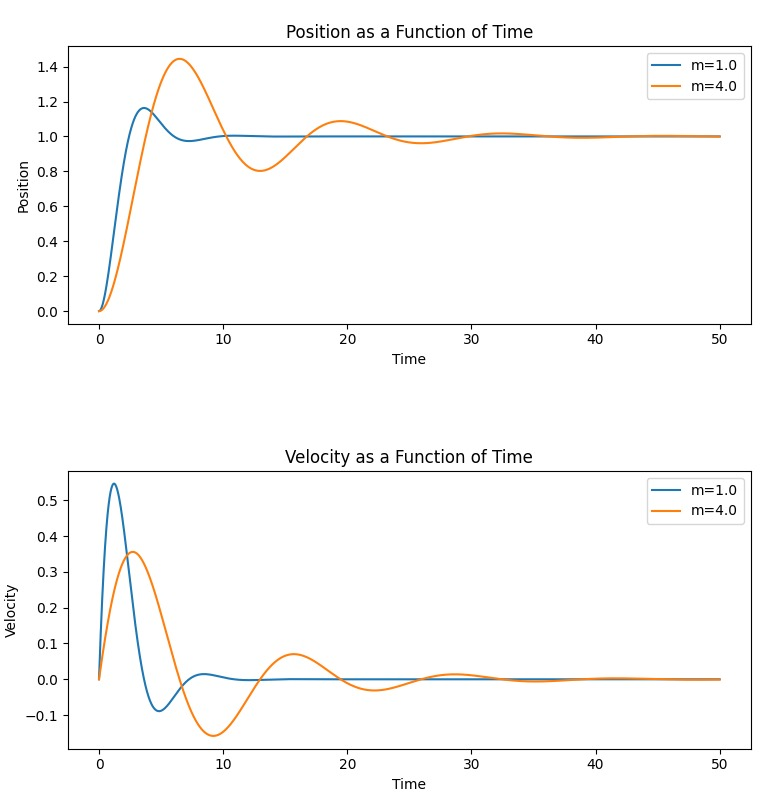
\includegraphics[width=\textwidth]{../assets/figure_1_mass.jpeg}
\caption{Posición - Velocidad en función del tiempo para distintos valores de masa, $t = 50$.}
\end{figure}


Este fenómeno se debe a que la fuerza aplicada, es constante, $F(t) = 1$, por lo que se necesita más tiempo para generar suficiente impulso y llegar al punto de equilibrio. Notar que en este caso al ser $t$ un límite de tiempo bajo, el sistema con mayor masa produce menos oscilaciones, puesto que la velocidad es menor y la amplitud es mayor.\\

Mismo experimento fue realizado pero aumentando el límite de tiempo 
$t$, mostró que el modelo con mayor masa presenta una mayor cantidad de oscilaciones antes de alcanzar el estado de equilibrio, como se puede ver en la figura 2.

\begin{figure}[H]
    \centering
    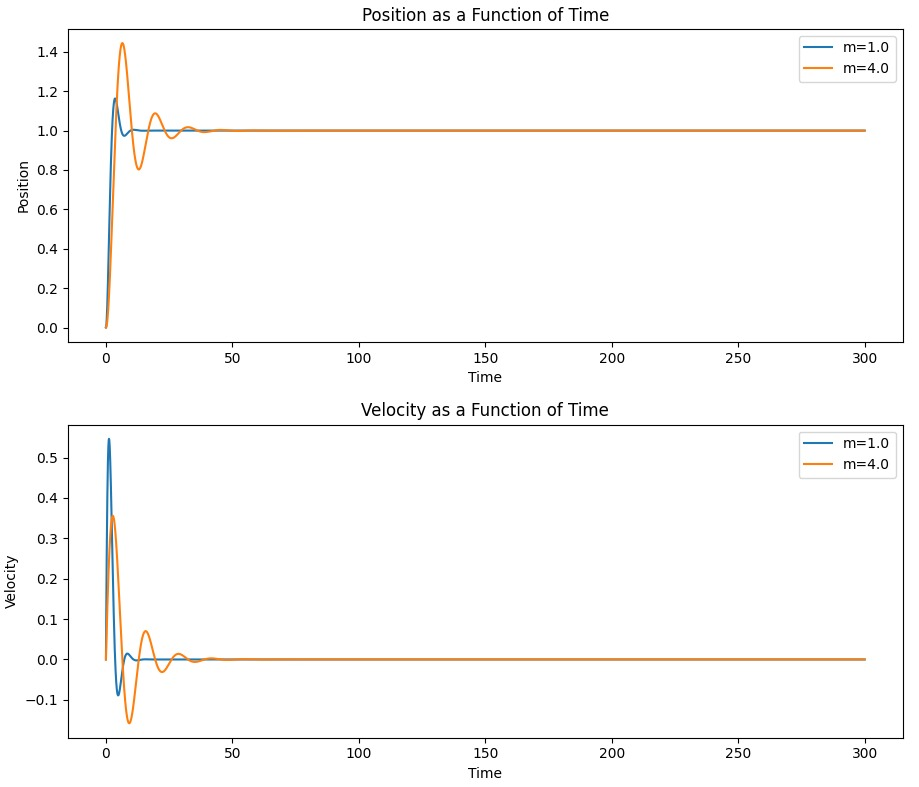
\includegraphics[width=\textwidth]{../assets/figure_3_mass.jpeg}
    \caption{Posición - Velocidad en función del tiempo para distintos valores de masa, $t = 300$.}
\end{figure}
    

Se presentan los resultados observados de la figura 1 y 2 junto con los datos de oscilacion, velocidad y posición en las tablas 2 3 y 4.
\captionsetup[table]{
  font=small,
  labelfont=bf,
  margin={1cm, 0cm}
}

\begin{table}[H]
    \caption{Resultados de la variación de la masa, el tiempo y las oscilaciones}
    \label{tab:mass_time_oscillations}
    \centering
    \begin{tabular*}{\textwidth}{@{\extracolsep{\fill}}|c|c|c|}
    \hline
    \textbf{Masa ($m$)} & \textbf{Tiempo Lim. ($t$)} & \textbf{Oscilaciones} \\
    \hline
    1.0 & 50 & 13 \\
    \hline
    4.0 & 50 & 7 \\
    \hline
    1.0 & 300 & 16 \\
    \hline
    4.0 & 300 & 36 \\
    \hline
    \end{tabular*}
\end{table}

\begin{table}[H]
    \caption{Resultados de la variación de la masa, el tiempo y la velocidad}
    \label{tab:mass_time_velocity}
    \centering
    \begin{tabular*}{\textwidth}{@{\extracolsep{\fill}}|c|c|c|c|}
    \hline
    \textbf{Masa ($m$)} & \textbf{Tiempo Lim. ($t$)} & \textbf{Vel. Máx.} & \textbf{Vel. Mín.} \\
    \hline
    1.0 & 50 & 0.546 & -0.089 \\
    \hline
    4.0 & 50 & 0.356 & -0.158 \\
    \hline
    1.0 & 300 & 0.546 & -0.089 \\
    \hline
    4.0 & 300 & 0.356 & -0.158 \\
    \hline
    \end{tabular*}
\end{table}

\begin{table}[H]
    \caption{Resultados de la variación de la masa, el tiempo y la posición}
    \label{tab:mass_time_position}
    \centering
    \begin{tabular*}{\textwidth}{@{\extracolsep{\fill}}|c|c|c|c|}
    \hline
    \textbf{Masa ($m$)} & \textbf{Tiempo Lim. ($t$)} & \textbf{Pos. Máx.} & \textbf{Pos. Mín.} \\
    \hline
    1.0 & 50 & 1.163 & 0 \\
    \hline
    4.0 & 50 & 1.444 & 0 \\
    \hline
    1.0 & 300 & 1.163 & 0 \\
    \hline
    4.0 & 300 & 1.444 & 0 \\
    \hline
    \end{tabular*}
\end{table}
A partir de los datos presentados en las tablas, se puede observar que el sistema con una mayor masa (4.0) presenta un mayor número de oscilaciones, velocidad máxima y mínima más baja, y una mayor distancia al punto de equilibrio  en  comparación con el sistema con menor masa (1.0). Esto refuerza la observación de que el sistema con una mayor masa tarda más tiempo en alcanzar el equilibrio y tiene una mayor amplitud de oscilación.

\subsection{Experimento 2: Ausencia de Fricción}

En este experimento, exploramos la dinámica del sistema en ausencia de fricción. Para ello, comparamos dos modelos que difieren solo en el coeficiente $b$:

\begin{itemize}
\item Modelo 1: $m = 1.0$, $k = 1.0$, $b = 1.0$, $F = 1.0$
\item Modelo 2: $m = 1.0$, $k = 1.0$, $b = 0.0$, $F = 1.0$
\item Simulación: $t = 300$, $\Delta t = 0.001$
\item Condiciones iniciales: $x(0) = 0.0$, $v(0) = 0.0$
\end{itemize}

El modelo 1, que incluye la presencia de fricción, presenta los resultados resumidos en la tabla 5.

\begin{table}[H]
    \caption{Resultados para el Modelo 1 con fricción}
    \label{tab:model_1_friction}
    \centering
    \begin{tabular*}{\textwidth}{@{\extracolsep{\fill}}|c|c|c|c|}
    \hline
    \textbf{Oscilaciones} & \textbf{Vel. Máx.} & \textbf{Vel. Mín.} & \textbf{Pos. Máx.} \\
    \hline
    16 & 0.546 & -0.089 & 1.163 \\
    \hline
    \end{tabular*}
\end{table}

El modelo 2, en ausencia de fricción, muestra los resultados en la tabla 6.

\begin{table}[H]
    \caption{Resultados para el Modelo 2 sin fricción}
    \label{tab:model_2_no_friction}
    \centering
    \begin{tabular*}{\textwidth}{@{\extracolsep{\fill}}|c|c|c|c|}
    \hline
    \textbf{Oscilaciones} & \textbf{Vel. Máx.} & \textbf{Vel. Mín.} & \textbf{Pos. Máx.} \\
    \hline
    95 & 1.000 & -1.000 & 2.000 \\
    \hline
    \end{tabular*}
\end{table}

De manera interesante, los resultados muestran que en ausencia de fricción, el sistema realiza más oscilaciones, alcanza velocidades más altas y posiciones más alejadas del equilibrio. 

Además, es importante destacar que en el modelo sin fricción y con una fuerza externa constante $F(t) = 1.0$, el sistema no converge a un estado de equilibrio, a diferencia de lo que se observa en sistemas con fricción. Este fenómeno se puede explicar en términos de la constante entrada de energía al sistema a través de la fuerza externa, que en ausencia de fricción no puede ser disipada.

Estas observaciones se vuelven más claras al analizar las gráficas de la posición y velocidad en función del tiempo para los dos modelos, que se muestran en la Figura 3. 

\captionsetup[figure]{
  font=small,
  labelfont=bf,
  margin={1cm,0cm}
}

\begin{figure}[H]
\centering
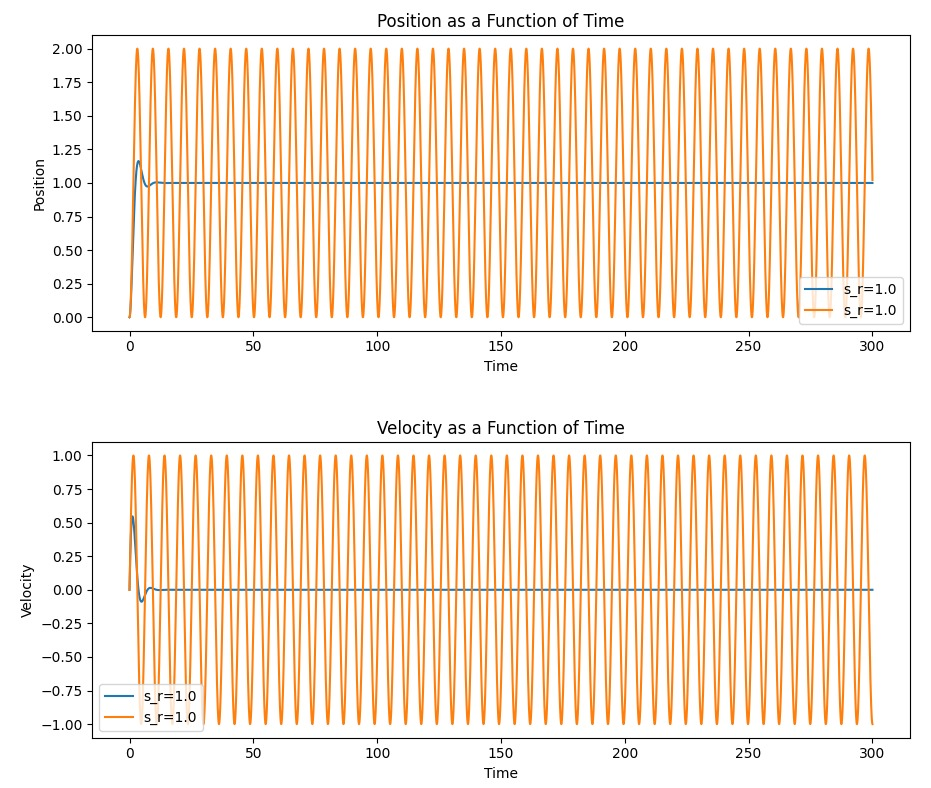
\includegraphics[width=\textwidth]{../assets/figure_2_friction.jpeg}
\caption{Posición y velocidad en función del tiempo para los modelos con y sin fricción.}
\end{figure}

Estos resultados resaltan el papel crucial de la fricción como mecanismo de disipación de energía que permite la convergencia al punto de equilibrio, limita las velocidades máximas y restringe las posiciones máximas que el sistema puede alcanzar.

\subsection{Experimento 3: Desplazamiento del estado de equilibrio}

En este experimento, investigamos el efecto de variar la fuerza $F$ en la dinámica del sistema. Mantuvimos los demás parámetros constantes, es decir:

\begin{itemize}
\item Masa, $m = 1.0$
\item Constante del resorte, $k = 1.0$
\item Resistencia al rozamiento, $b = 1.0$
\item Posición inicial, $x_0 = 0.0$
\item Velocidad inicial, $v_0 = 0.0$
\end{itemize}

Luego, implementamos simulaciones con distintos valores de fuerza, en particular $F = 1.0$, $F = 2.0$ y $F = 3.0$.\\

Los resultados de las simulaciones para cada valor de fuerza se resumen en la tabla \ref{tab:force_results}.

\begin{table}[H]
    \caption{Resultados para distintos valores de fuerza}
    \label{tab:force_results}
    \centering
    \begin{tabular*}{\textwidth}{@{\extracolsep{\fill}}|c|c|c|c|c|}
    \hline
    \textbf{Fuerza ($F$)} & \textbf{Oscilaciones} & \textbf{Vel. Máx.} & \textbf{Vel. Mín.} & \textbf{Pos. Máx.} \\
    \hline
    1.0 & 13 & 0.546 & -0.089 & 1.163 \\
    \hline
    2.0 & 13 & 1.093 & -0.178 & 2.326 \\
    \hline
    3.0 & 13 & 1.639 & -0.267 & 3.489 \\
    \hline
    \end{tabular*}
\end{table}

Los resultados muestran que al  aumentar la fuerza que se aplica se incrementa tanto la velocidad máxima como la posición máxima alcanzada por el sistema, sin alterar el número de oscilaciones.\\

El efecto de la variación de la fuerza se puede visualizar en la figura \ref{fig:force_results}, que muestra la posición y la velocidad en función del tiempo para los distintos valores de fuerza.

\captionsetup[figure]{
  font=small,
  labelfont=bf,
  margin={1cm,0cm}
}

\begin{figure}[H]
\centering
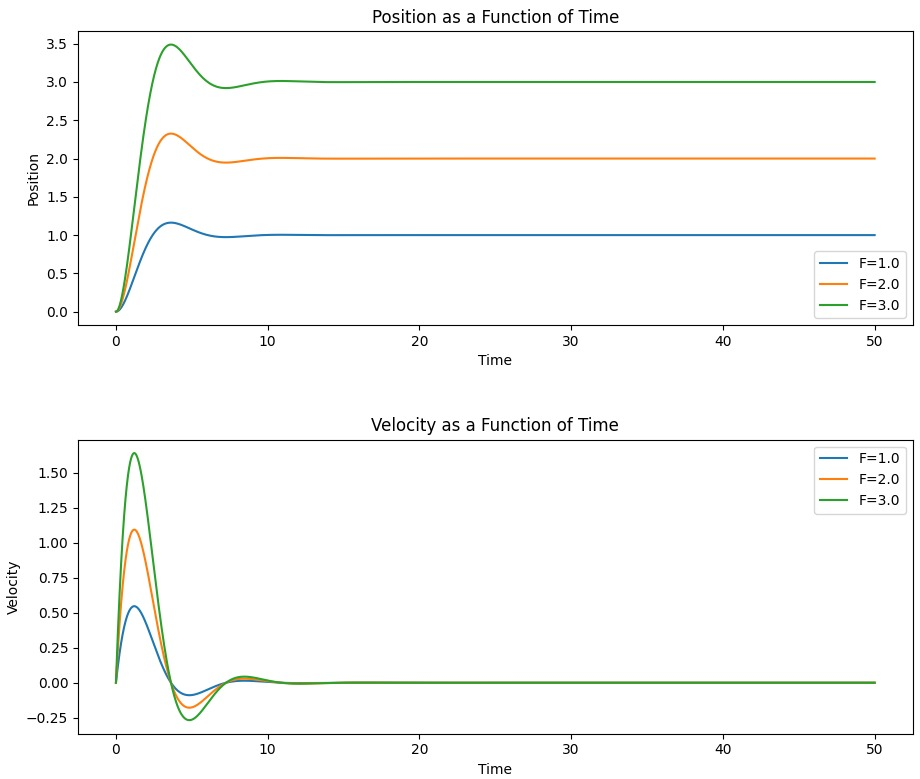
\includegraphics[width=\textwidth]{../assets/figure_1_force.jpeg}
\caption{Posición - Velocidad en función del tiempo para distintos valores de fuerza.}
\label{fig:force_results}
\end{figure}

Estos resultados indican que aumentar la fuerza aplicada al sistema puede ser una forma efectiva de aumentar tanto la velocidad como la distancia que el sistema puede alcanzar como se discutió anteriormente, también es importante destacar que al ser $F(t)$ constante el punto de equilibrio del sistema se desplaza, como se puede observar en la figura \ref{fig:force_results}.

\section{Conclusiones}
En este estudio, investigamos la dinámica de un sistema oscilatorio \textit{masa-resorte} bajo la influencia de una serie de parámetros, incluyendo la masa del objeto, la resistencia al rozamiento, la fuerza externa, y las condiciones iniciales de posición y velocidad. 
Al final de cada experimento se realizó una conclusión sobre los resultados obtenidos, resumidamente destacamos:

\begin{itemize}
\item Aumentar la masa del objeto requiere un mayor tiempo $t$  para alcanzar el punto de equilibrio y este aumento de masa ocasiona una mayor amplitud de oscilación. Este resultado se deriva de la mayor inercia presentada por el objeto, lo que requiere más impuslo para moverlo.
\item La fricción desempeña un papel crucial en la disipación de la energía del sistema, permitiendo su convergencia al punto de equilibrio. En ausencia de fricción, observamos que el sistema realizaba más oscilaciones, alcanzaba velocidades más altas, y lograba posiciones más alejadas del equilibrio. En particular, un sistema sin fricción y con una fuerza externa constante $F(t)$ no converge a un estado de equilibrio, ya que la energia no puede ser disipada.
\item Al variar la fuerza externa, descubrimos que aumentarla resulta en un incremento en la velocidad máxima y  posición máxima, sin alterar el número de oscilaciones. No obstante, al ser $F(t)$ constante el punto de equilibrio del sistema se desplaza, como se pudo observar en el experimento debatido en la seccion anterior.
\end{itemize}

Conclusiones más detalladas se pueden encontrar en la sección 4 de este informe, a través de cada experimento realizado.

\end{document}
